\section{Numerical Analysis}
Although one certainly would have some intuition about how the potential distribution should look like if the distribution had lesser number of charge distributions, the intuition tends to be not so reliable in complex systems. Therefore it becomes natural to approach computaional methods for help. The computaional results themselves have to be judged, one way to do so is a brief check that the result vaguely approximates our intuition, another method is by employing different computaional methods to make sure that the method is not biased to a particular solution. For example, if SOR produces a wildly different solution than Jacobi or the former takes more number of iterations than later then certainly either one of the solvers is wrongly implemented. Before we move on to analysing the various results we obtained using the different solving methods, we will first establish the intuitive expectations that we first put forward while framing the problem and before obtaining the final results. Later we will have a short discussion about the role discritization plays in our solution.

\subsection{Expectations}

To remind ourselves, our problem consists of an interleaved capacitor which is charged to a potential of $\pm5 V$ and then disconnnected. In our problem the first plate $A_{1}$ and the last plate $A_5$ of the capacitor were maintained at $+5V$. We are solving our problem assuming perfect symmetry along the third direction that is along the surface of the plates.(the z-direction).

\begin{figure}[ht]
    \centering
    \def\svgwidth{0.6\textwidth}
    \import{./diagrams}{analysis.pdf_tex}
    \caption{This diagram represents the region $\omega$ being studied, $\alpha_1,\alpha_2,\alpha_3,\alpha_4$ are the only unique regions in $\omega$ that were analysed.}
    \label{}
\end{figure}
\begin{itemize}
    \item \textbf{Symmetry: } Now since in our arrangement is symmetrical, the resulting solution obtained should also be symmetrical about the line $x = 2$. 
    \item High Potential near the positively charged plates (i.e. the plates denoted by A  in the figure1) of capacitor and low potential near the negatively charged plates but we are considerig them in two dimension so they will behave as the "line charge distributions. Since we are ensuring the value at the boundary reamins constant at $ +5 volts $ so the distribution should contain a positive spike in value of potential at the location of $A_i$  having positive potential at the beginning and negative spike at places of negative potential
    \item  In region $ \alpha_2 $ potential is fixed at $ + 5 volts $ at $ x = 0 $ and stretches to $ x = 0.5 $ where $ B_1 $ was initially charged with $ - 5 volts $. We expect to see a decline in potential in region $ \alpha_2 $ due to initial conditions across x direction.
    \item The  $ B_1 $ plate extends for $ y \in (0.4, 4.4)  $ so we expect to see concentration of negative charges hence negative potential  for  higher values  of y where initially there was presence of negatively charged potential plate $ B_1 $ and a comparitively higher potential for $ \alpha_1 $ or lower values of y because it is surrounded by two positively charged plates.
    \item for region $ \alpha_3   $  we expect to see a rise  in potential from $ x = 0.5 $ to $ x = 1 $  because it is surrounded by negatively charged potential plate at $ x = 0.5 $ and postively charged plate at  $ x = 1 $.
    \item The plate $ A_2 $ ends at the boundary of $ \alpha_4 $ and it is surrounded by two negatively charged plates on both sides so we expect to see a concentration of negatively charged potential in region $ \alpha_4 $.
    \item For region $ x \in (1 , 1.5) $ the trend should be similar to region $ \alpha_2 $ and for region $ x \in (1.5, 2) $ we expect  trend to be similar to $ \alpha_4 $ . 
    \item Now due to symmetry we expect to see the potential distribution after $ x = 2 $ same as before it with the line $ x = 2 $ as mirror
\end{itemize}

\subsection{Results}
Now that we have converted the problem into a system of linear equations by applying the relation \ref{eq:difference equation} to each node on the mesh and analysed the conversion, we move on to analyse the computational results obtained using three different iterative methods namely Jacobi, Gauss-Seidel and S.O.R to solve the system of linear equations.


\begin{figure}[ht]
    \centering
    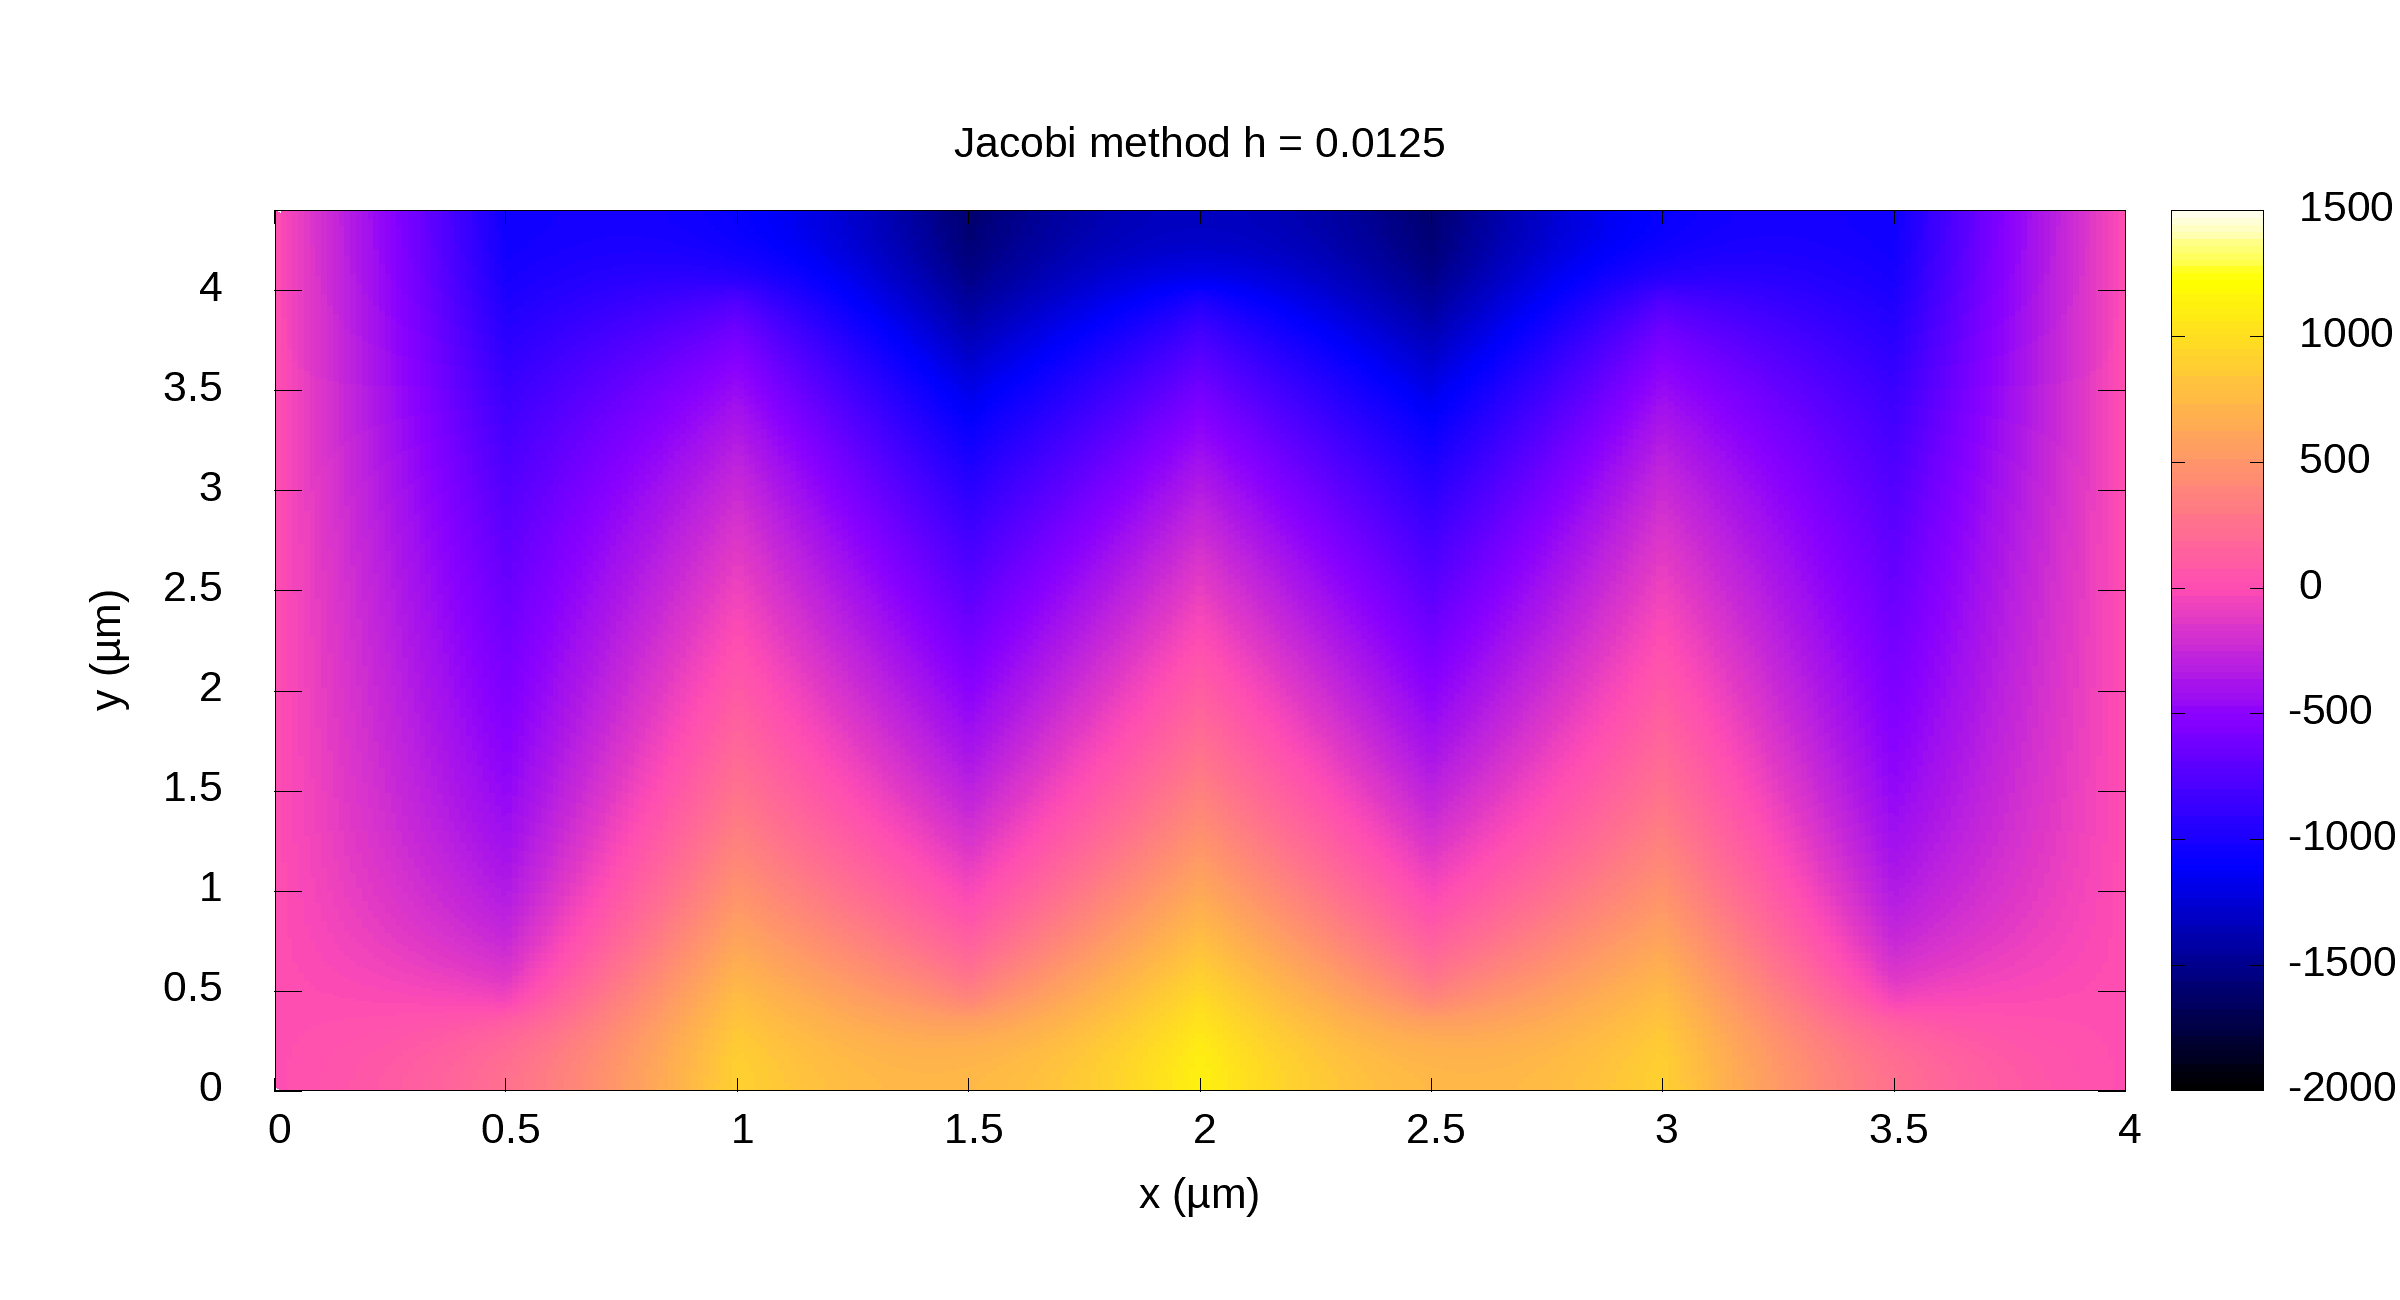
\includegraphics[height= 70mm]{content/graphs/Jacobi_0125_map.png}
    \caption{Jacobi}
    \label{fig1}
\end{figure}%

\begin{figure}[ht]
    \centering
    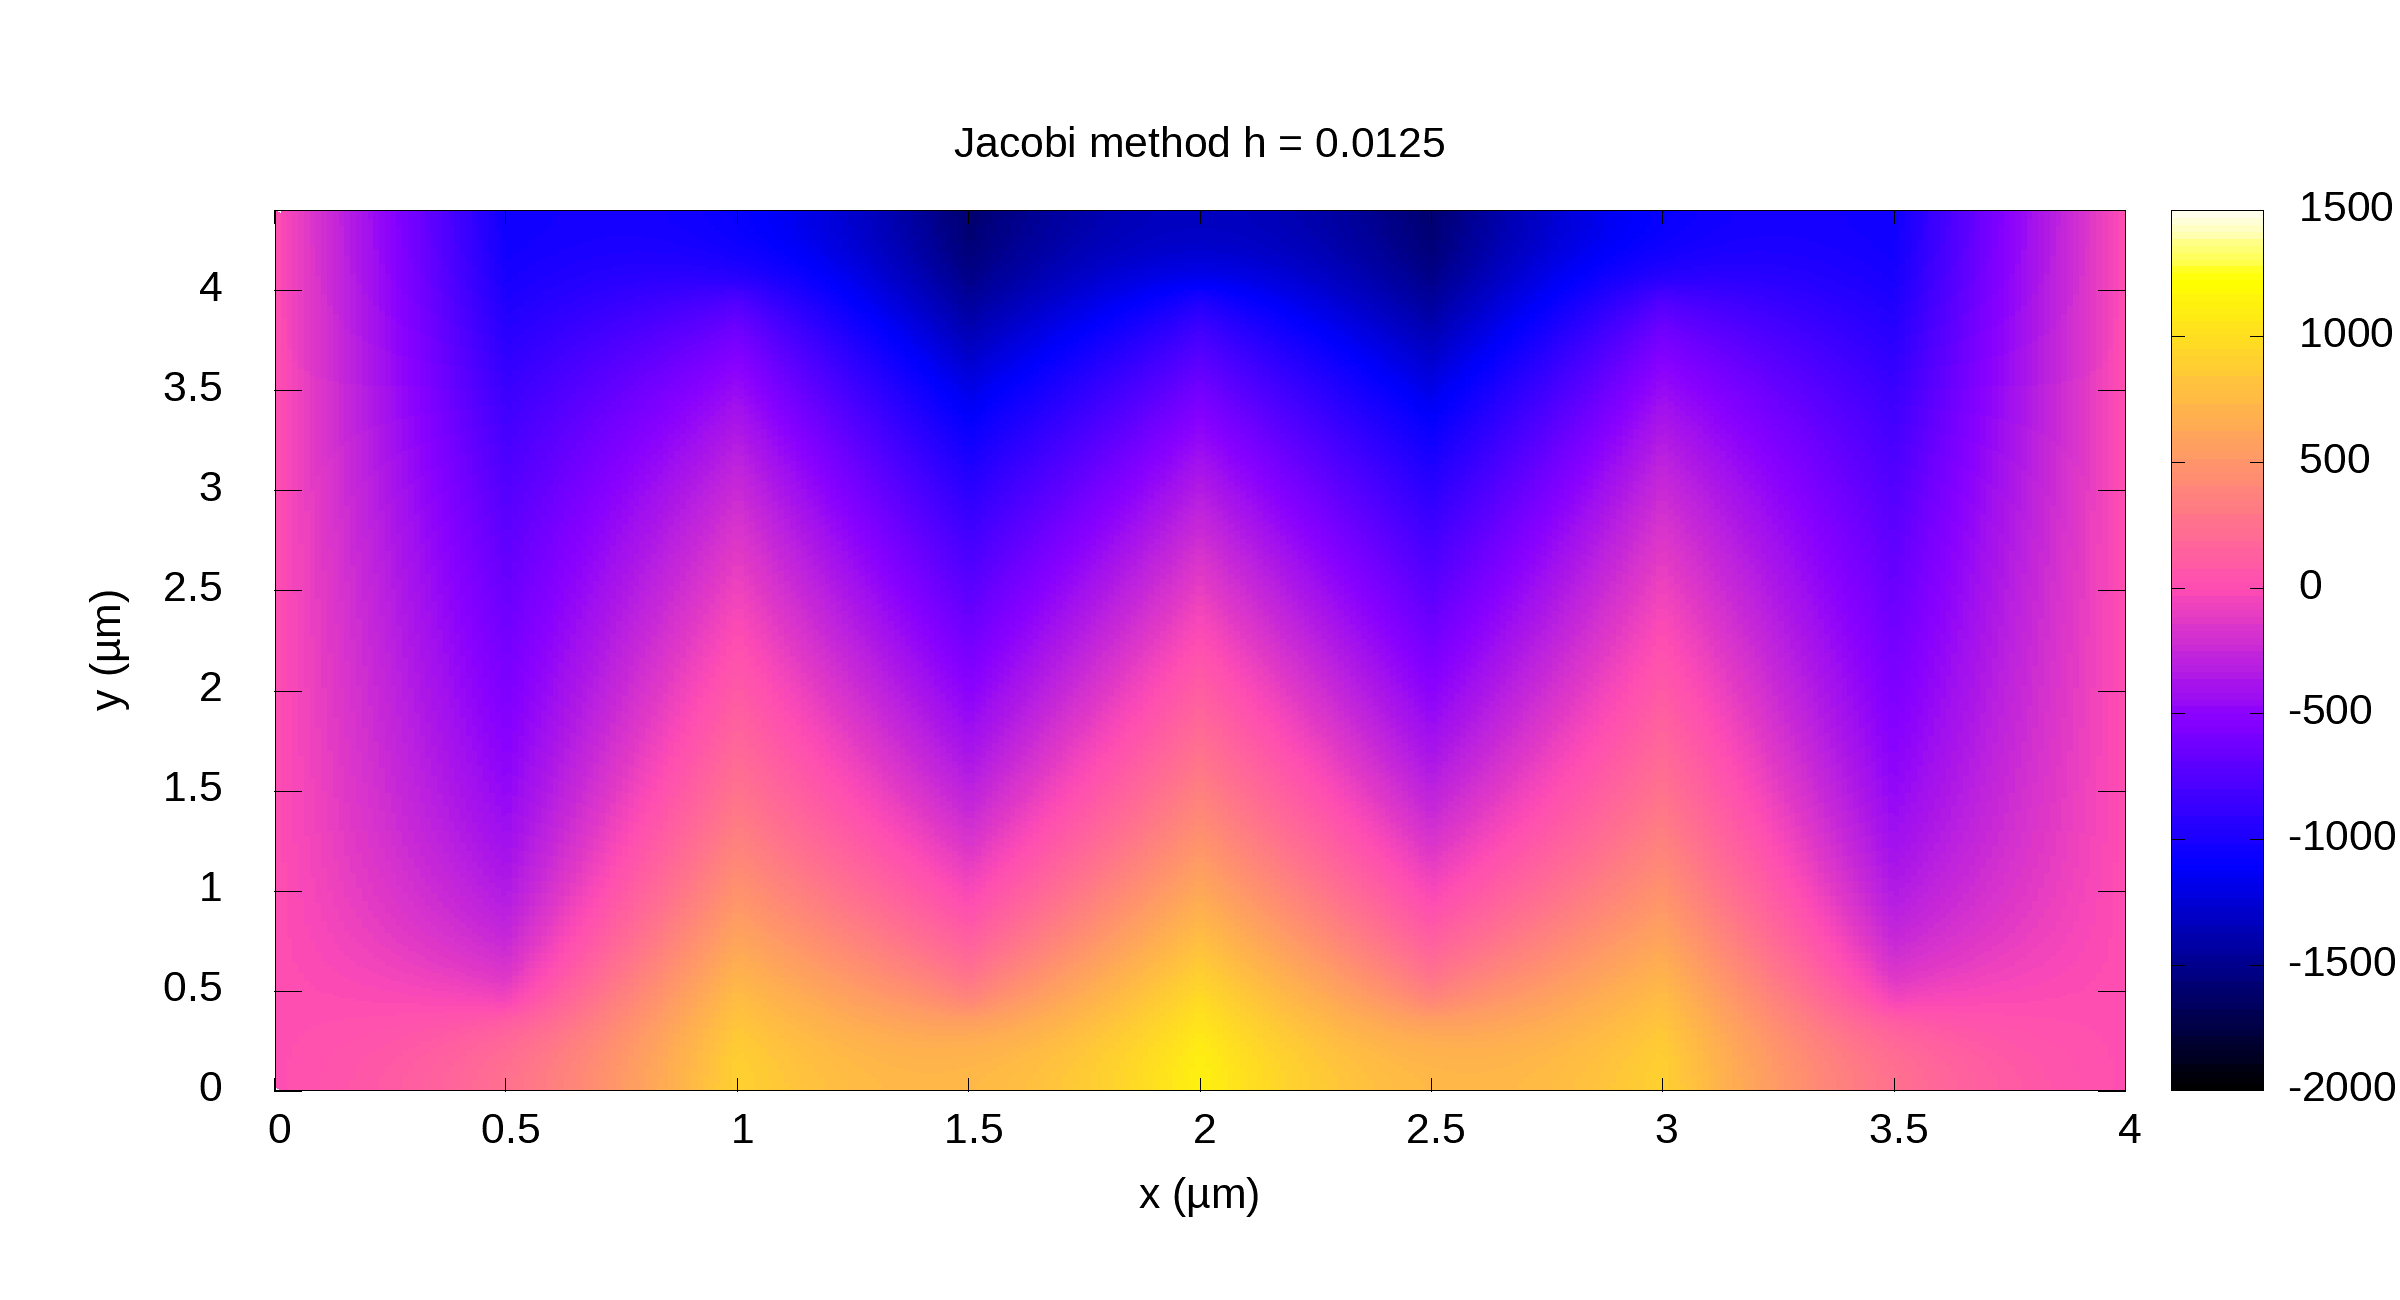
\includegraphics[height= 70mm]{content/graphs/Jacobi_0125_map.png}
    \caption{Jacobi}
    \label{fig2:}
\end{figure}%
\begin{figure}[ht]
    \centering
    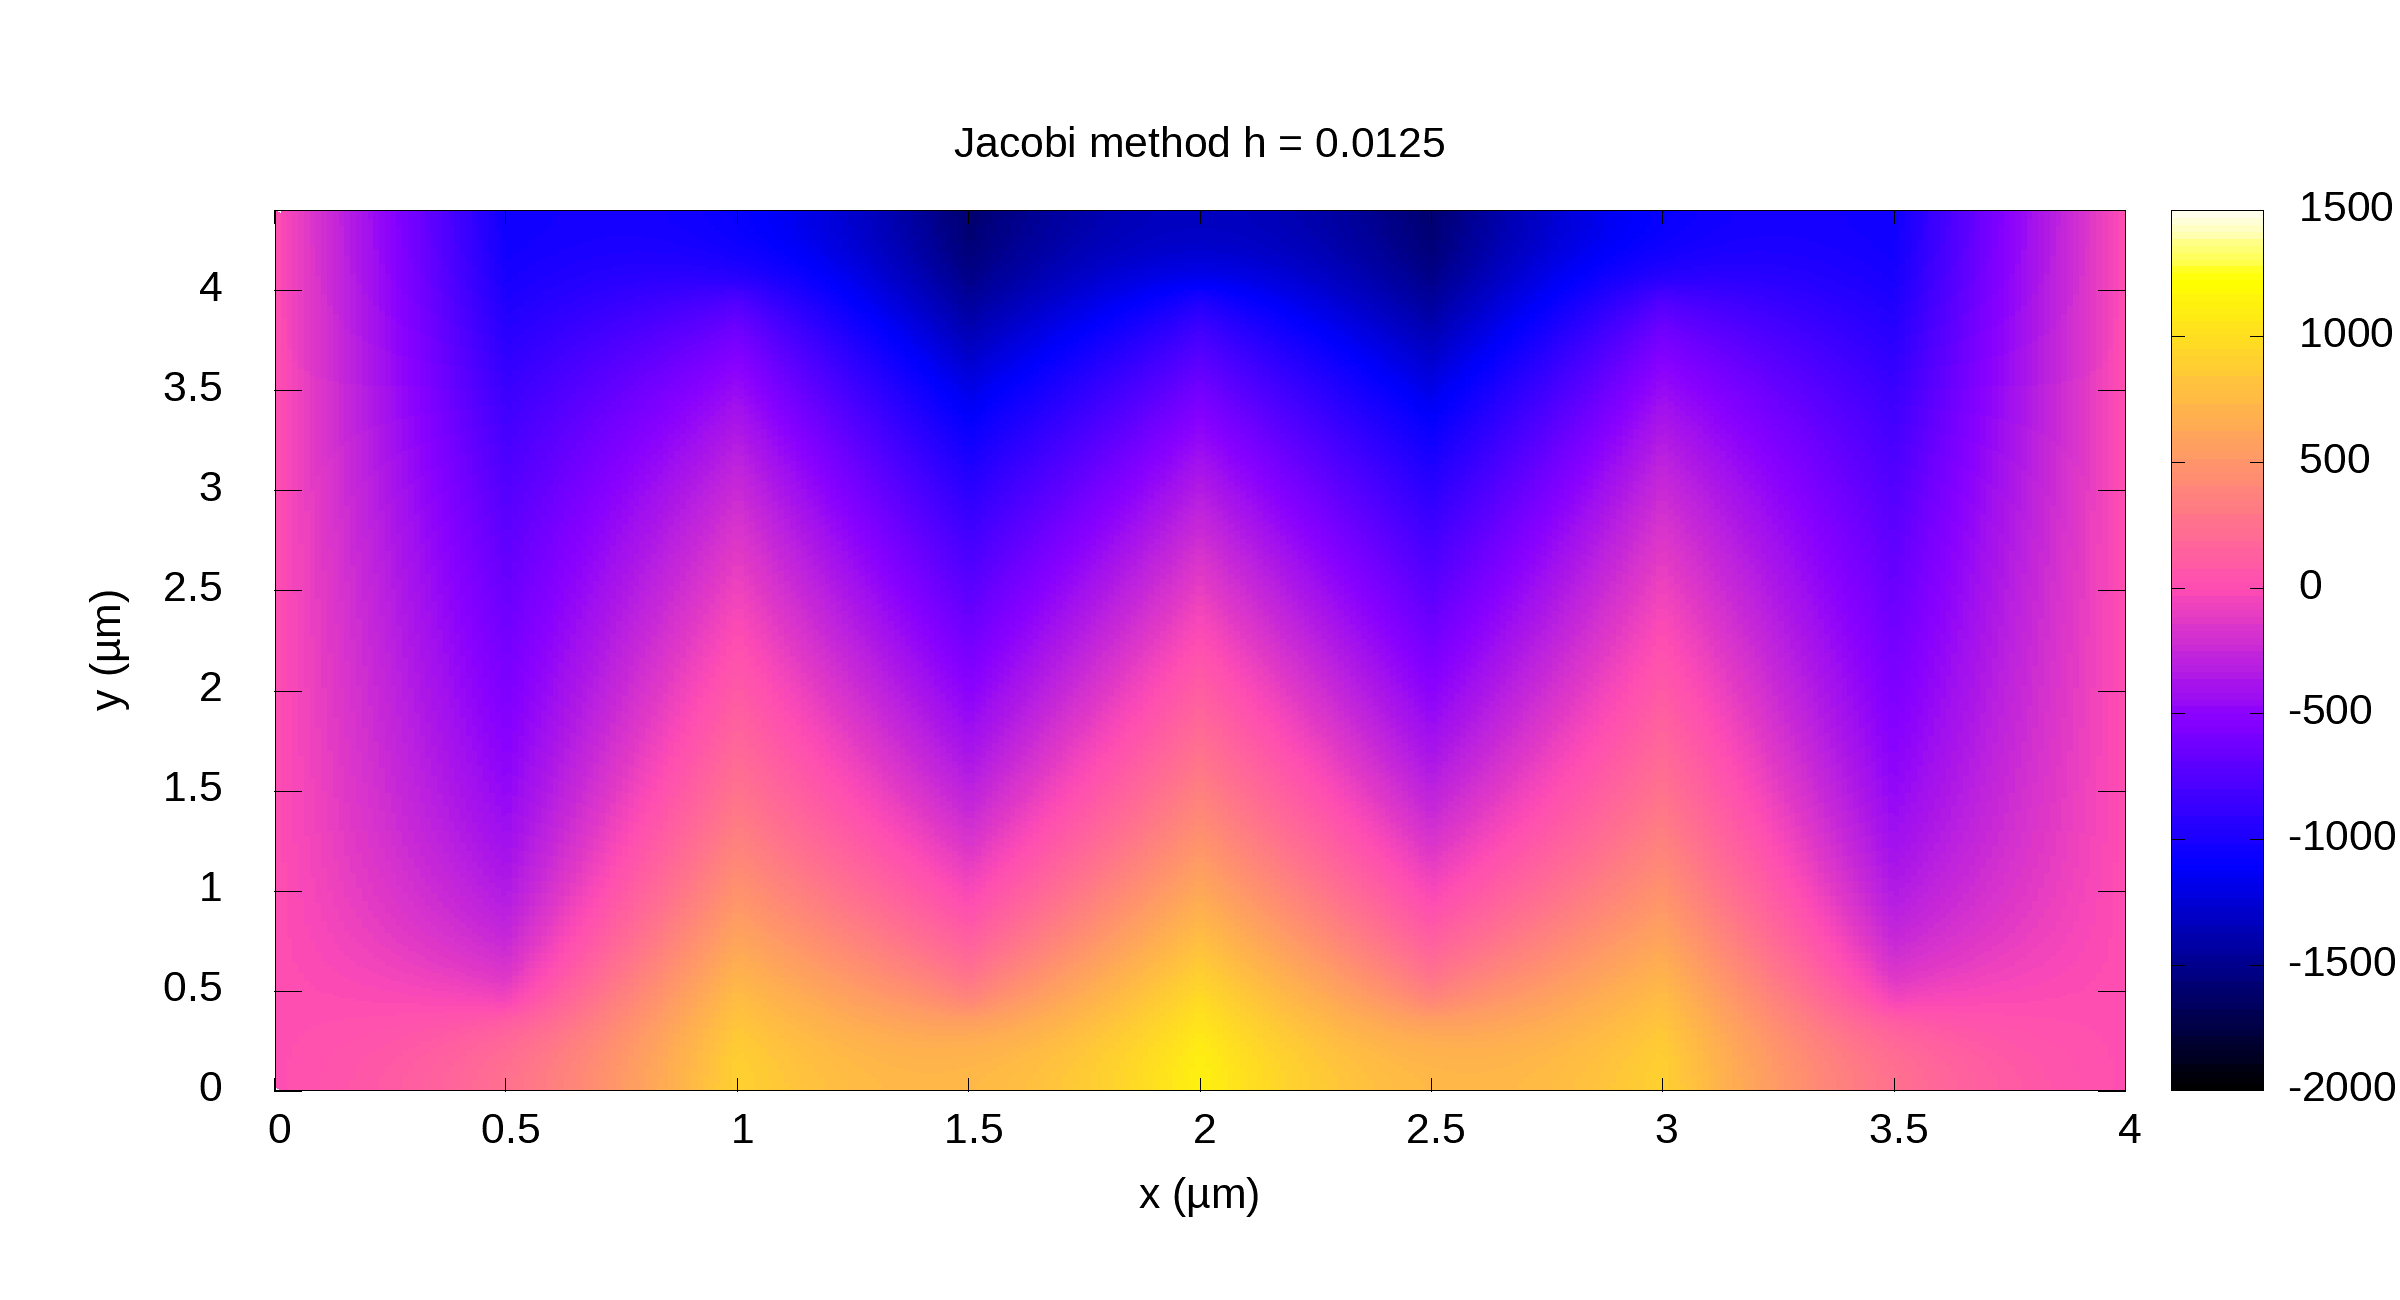
\includegraphics[height= 70mm]{content/graphs/Jacobi_0125_map.png}
    \caption{Jacobi}
    \label{fig3:}
\end{figure}%

\paragraph{Comparison of Method}{%
Since all the iterative methods we used have given us almost identical results so we will only compare them on the basis of number of iteration required so as to determine which method is more compuationally cheap and viable}
    
\begin{table}[ht]
    \centering
    \begin{tabular}{|c|c|c|c|}
    \hline
    \multirow{2}{*}{\gs\gs meshsize $h$ \gs\gs} & \multicolumn{3}{c|}{No. of iterations}  \\ \cline{2-4}
                                    & \gs \gs Jacobi \gs \gs & \gs \gs Gauss-Seidel \gs\gs & \gs S.O.R (1.9) \gs \\ \hline
    0.01                                &11878& 6315& 251\\ \hline
    0.05                                &52047& 26983 &1552\\ \hline
    0.025                               &182367&94927&5821\\ \hline
    0.0125                              &674230&335520 &22163 \\ \hline
\end{tabular}
\caption{\centering Table comparing the number of iterations required for each method for a relative tolerance of $10^{-8}$}
\label{iterations}
\end{table}


\begin{table}[ht]
    \centering
    \begin{tabular}{|c|c|c|c|}
    \hline
    \multirow{2}{*}{\gs\gs meshsize $h$ \gs\gs} & \multicolumn{3}{c|}{Approximate computation time ($\pm 0.01s$)}  \\ \cline{2-4}
                                    & \gs \gs Jacobi \gs \gs & \gs \gs Gauss-Seidel \gs\gs & \gs S.O.R (1.9) \gs \gs   \\ \hline
    0.01                                &0.41&0.27&0.02\\ \hline
    0.05                                &6.13& 3.96&0.28\\ \hline
    0.025                               &90.73&55.46&3.47 \\ \hline
    0.0125                              &1380.54&818.68&54.35\\ \hline
\end{tabular}
\caption{\centering Table comparing the computation time required for each method for a relative tolerance of $10^{-8}$}
\label{computation_time}
\end{table}

\subsubsection{Successive Over Relaxation (SOR)}
In this section we analyse the results obtained for different values of relaxation factor. \\[2mm]
\noindent
\textbf{ Optimum value of Relaxation Factor } \\
In Successive Over Relaxation we have to choose the value of a relaxation factor which is responsible for the rate of convergence of solution. It's value can be chosen anywhere between 1 to 2 i.e. relaxation factor or $\omega  \in [1,2]$. We observed the variation of No. of iterations required to reach a given tolerance with change in $ \omega $. The following graph represents the graph between number of itereations and value of $\omega$. \\
\begin{figure}[ht]
    \centering
    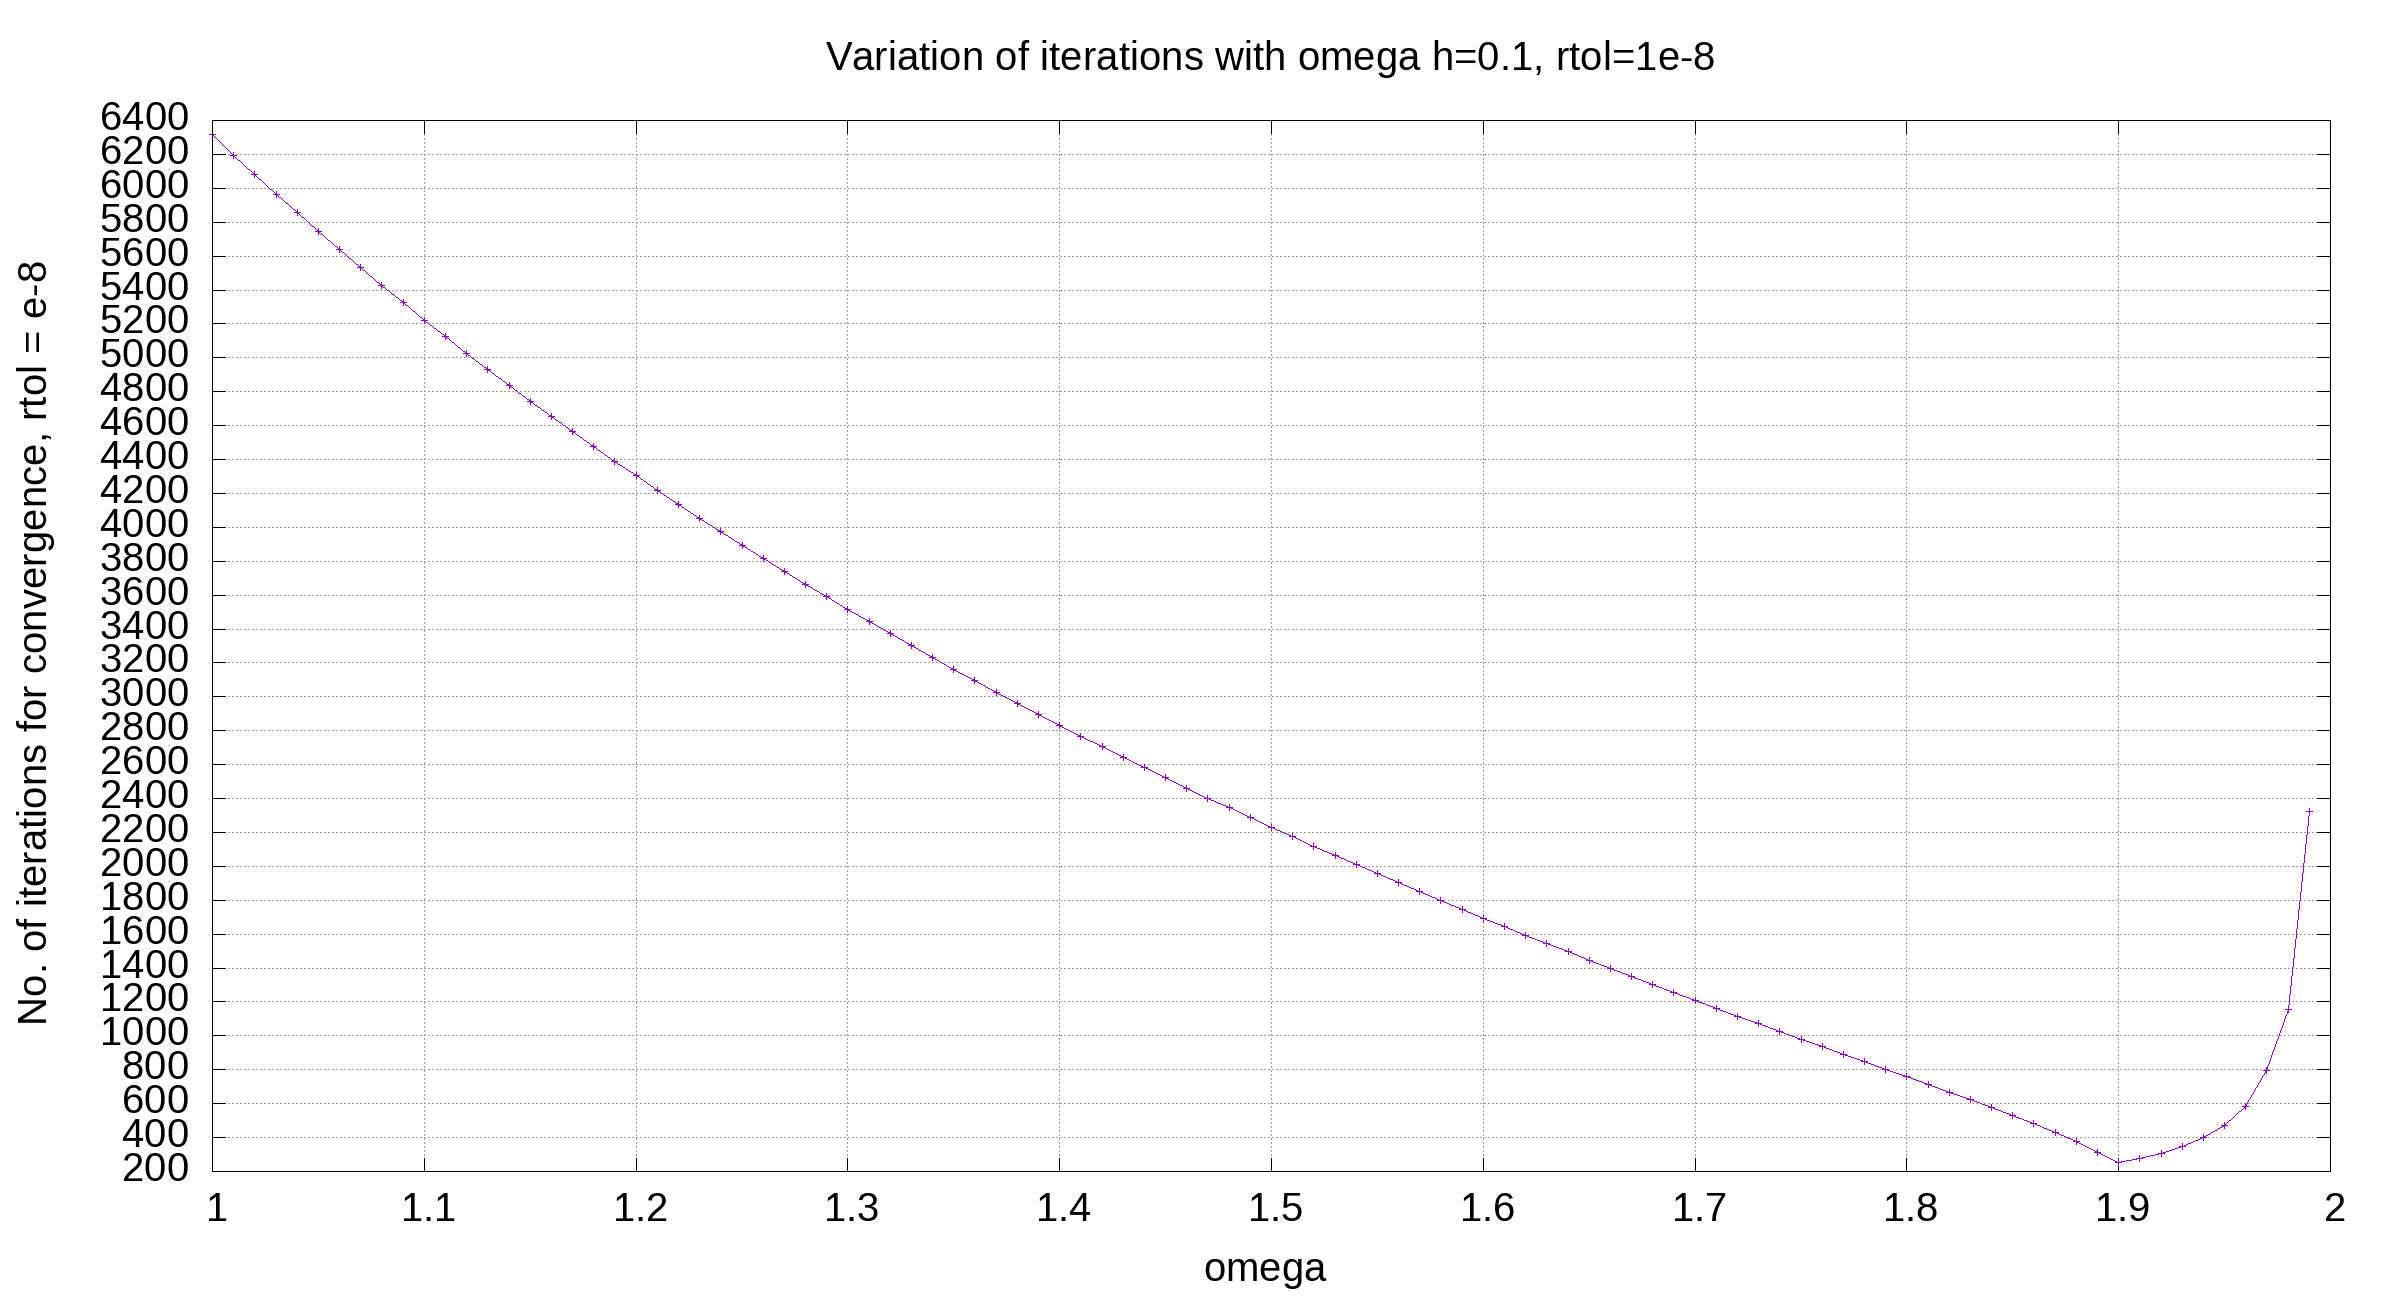
\includegraphics[width=\textwidth]{content/graphs/omega.png}
    \caption{variation of number of iterations for convergence with relative tolerance=$10^{-8}$ and meshsize $h = 0.1$  }
    \label{omega variation}
\end{figure}
From the graph we can see that the most optimum value of $ \omega $ is $1.89$ according to number of iterations required to reach the solution.Now we will analyse the plot, heat map and  compare it with the expectation. The below figure shows the heat map and the 3d plot of solution. \\

So comparing all the method for computation under identical condition on the basis of number of iteration required for acheiving the required tolerance we can say $ \boldsymbol{SOR Method} $ is best method among all three iterative schemes used.
\newpage
\section{Conclusion}
\subsection{Result}
We tried to solve the problem of interleaved capacitor using the finite difference method for solving poisson equation. We have solved the problem using three different iterative schemes. After completing this project we can say that the method of SOR is best for solving the system of linear equation after using the finite differences method. Using SOR method we were able to solve mesh of size $ (480 times 480) $ in just $ xxxxxx $ number of iteration in just $  yyyy $ seconds. Also we gained good insight and intuition after solving the problem of interleaved capacitor.
\subsection{Experience}
We learnt a lot of new things during this project. We have gained the knowledge on how to solve a physical problem computationally and the various process involved in it such as non-dimensionalisation, the concept of convergence etc. Our python, latex and gnu skills have also increase significantly and our fascination with power of poisson equation and computation method have only gone uphill as compared to start of project of how one can solve such complex physical problem just by using some standard method and understand the "physical aspect " of such problems easily. We also spend a good portion of time studying about theoretical aspects of different computational methods and trying to understand the concepts about which we didn't pay a lot of attention to earlier such as the truncation error , round off error etc. This project has been an incredible journey for us as it has not only increased our theoretical , physical and compuational knowledge but it has also taught us about the importance of perseverance and patience as there were many topic or subtopics that we didn't understand easily just by studying about it from one or two place or things that were not easily available in comprehendable nature for us due to advance nature of partial differential equation and sometimes we have to spend a lot of time just searching about it. But in the end we are very grateful that we had chosen such a topic that has taught us so much. 
\end{document}